%% \union - Example: \union{j \in J}{A_j}
\newcommand{\union}[2]{\underset{#1}\bigcup #2}

%% \inter - like \union, but with \bigcap
\newcommand{\inter}[2]{\underset{#1}\bigcap #2}

\newcommand{\rad}{\text{rad }}
\newcommand{\rom}{\mathbf{R}^m}
\newcommand{\rl}{\mathbf{R}}
\newcommand{\countable}{
    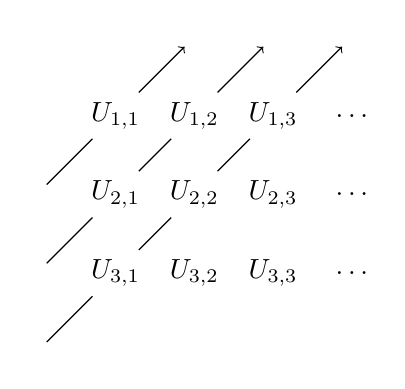
\begin{tikzpicture}[align=center]
        \label{pics}
        \node(n02) at (2,0) {};
        \node(n03) at (3,0) {};
        \node(n04) at (4,0) {};
        \node(n11) at (1,-1) {$U_{1,1}$};
        \node(n12) at (2,-1) {$U_{1,2}$};
        \node(n13) at (3,-1) {$U_{1,3}$};
        \node(n14) at (4,-1) {$\dots$};
        \node(n20) at (0,-2) {};
        \node(n21) at (1,-2) {$U_{2,1}$};
        \node(n22) at (2,-2) {$U_{2,2}$};
        \node(n23) at (3,-2) {$U_{2,3}$};
        \node(n24) at (4,-2) {$\dots$};
        \node(n30) at (0,-3) {};
        \node(n31) at (1,-3) {$U_{3,1}$};
        \node(n32) at (2,-3) {$U_{3,2}$};
        \node(n33) at (3,-3) {$U_{3,3}$};
        \node(n34) at (4,-3) {$\dots$};
        \node(n40) at (0,-4) {};
        \draw(n20) -- (n11);
        \draw[->](n11) -- (n02);
        \draw(n30) -- (n21);
        \draw (n21) -- (n12);
        \draw[->](n12) -- (n03);
        \draw(n40) -- (n31);
        \draw (n31) -- (n22);
        \draw (n22) -- (n13);
        \draw[->](n13) -- (n04);
    \end{tikzpicture}
}